\section{Grundlagen} % (fold)
\label{sec:grundlagen}

	% \subsection{Röntgenstrahlen} % (fold)
	% \label{sub:röntgenstrahlen}

	% 	Gefährlich, aber können witzige Punkte auf Photopapier hinterlassen.
	% 	Auch x-Rays genannt.
	% 	Wurden im Jahre 1903 von Charles X. Xavier (alias Prof. X) im Cerebro erzeugt.
	% 	Weniger Energie als Gamma-Strahlen.
	% 	Deswegen wird man auch nur klein und grün bei längerer Bestrahlung anstatt groß und grün.
	% 	Vergleiche --> Hulk.
	% % subsection röntgenstrahlen (end)


	% \subsection{Kristalle} % (fold)
	% \label{sub:kristalle}

	% 	Durchsichtig, meist eckig und teuer.
	% 	Kommen vor allem in Truhen und Dungeons bei "Bossen" vor.
	% 	Nicht zu verwechseln mit Crystal (vgl. --> Meth).
	% % subsection kristalle (end)


	\subsection{Erzeugung von Röntgenstrahlung} % (fold)
	\label{sub:erzeugung_von_rntgenstrahlung}

		Röntgenstrahlung bezeichnet elektromagnetische Wellen mit Energien im Bereich von $10^{0}$ bis $10^3\unit{keV}$ und demnach einen entsprechenden Wellenlängenbereich von $10^{-3}$ bis $10^0\unit{nm}$.
		Röntgenstrahlen liegen im elektromagnetischen Spektrum zwischen dem ultravioletten Licht und der Gammastrahlung, mit der sie sich teilweise überschneiden.
		Sie besitzen sowohl Teilchencharakter, welcher durch das Auftreten des Compton- oder Photoeffekts gezeigt wird, als auch die für diesen Versuch relevanten Welleneigenschaften, wie zum Beispiel die der Beugung an Kristallgittern.

		Vor Allem für diese Strahlungsart lässt sich die Beugung an Kristallgittern besonders gut beobachten, weil die Wellenlänge von Röntgenstrahlen eine ähnliche Größenordnung besitzt wie die Gitterkonstanten eines Kristalls.
		Diese liegt im Bereich von einigen Pikometern.

		Im Versuch wird die benötigte Röntgenstrahlung hauptsächlich durch zwei Mechanismen erzeugt.
		Beide Vorgänge finden in der sogenannten Röntgenröhre statt.

		\subsubsection{Röntgenbremsstrahlung} % (fold)
		\label{ssub:rntgenbremsstrahlung}

			\urldef{\refRoehre}\url{https://lp.uni-goettingen.de/get/image/6621}
			\urldef{\refIntensity}\url{http://users.physik.fu-berlin.de/~wbrewer/IMAGES/ronts.jpg}

			In einer Röntgenröhre, wie sie in Abbildung \ref{fig:roehre-scheme} zu sehen ist, treffen stark beschleunigte Elektronen ($10$ bis $100 \unit{keV} $) auf eine Metallanode.
			Dort werden sie auf einer sehr kurzen Strecke abgebremst und übertragen somit, wie aus der Elektrodynamik bekannt, einen Teil ihrer Energie auf ein Photon, welches emittiert wird.
			Je nachdem wie stark und auf welche Weise und in welchem Material die Ladungsträger abgebremst werden, entstehen unterschiedlich energiereiche Röntgenquanten.
			Das Spektrum der Röntgenröhre ist somit kontinuierlich.
			Abbildung \ref{fig:roehre-intensity} zeigt die Intensitätsverteilung der verschiedenen Wellenlängen für unterschiedliche Anodenspannungen $U_\m{A}$.
			
			\begin{figure}[htb]
				\centering
				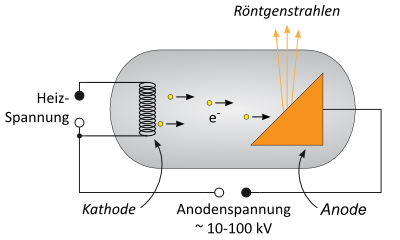
\includegraphics[scale = 1]{images/roehre-schema.png}
				\caption{grundsätzlicher Aufbau einer Röhre zur Erzeugung von Röntgenstrahlung \\ Quelle: \refRoehre}
				\label{fig:roehre-scheme}
			\end{figure}
			
			\begin{figure}[htb]
				\centering
				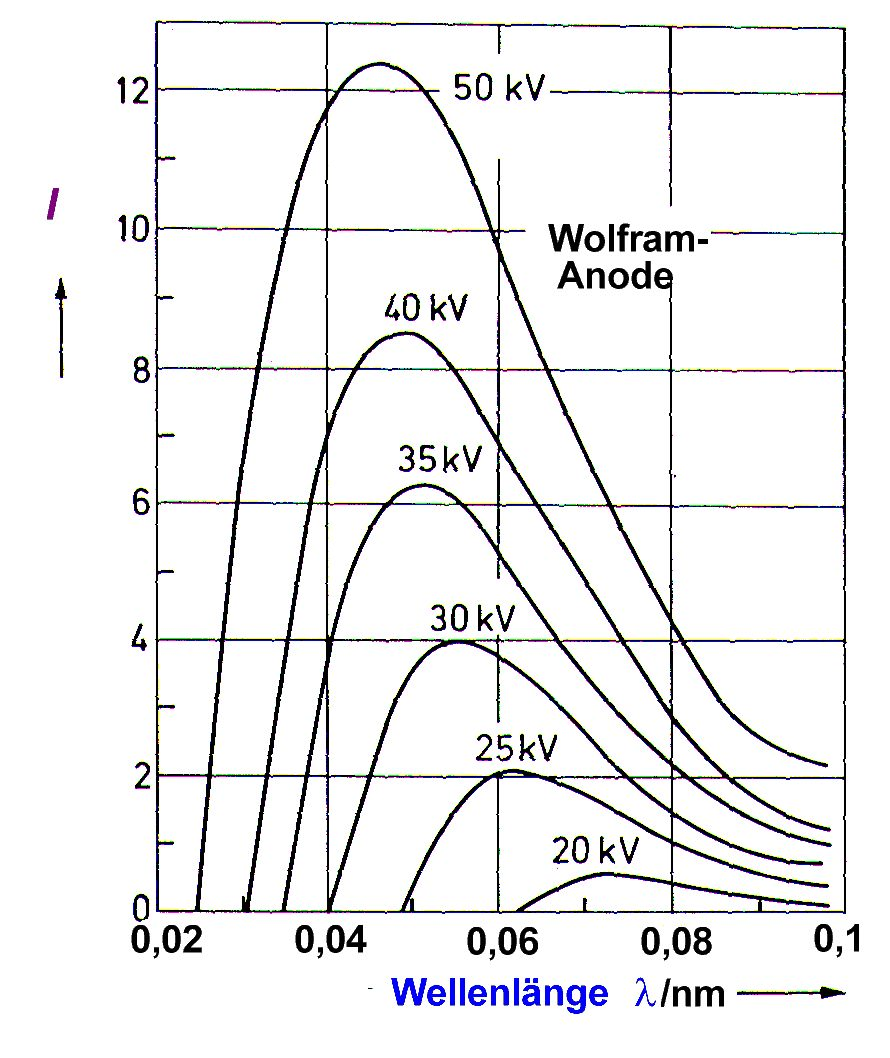
\includegraphics[scale = 0.8]{images/bremsstrahlung.jpg}
				\caption{Intensitätsverteilung der durch eine Röhre erzeugten Röntgenbremsstrahlung für verschiedene Anodenspannungen \\ Quelle: \refIntensity}
				\label{fig:roehre-intensity}
			\end{figure}

			Im Allgemeinen steigt die Intensität der ausgesendeten Röntgenstrahlung mit der Kernladungszahl des Anodenmaterials.
			Abbildung \ref{fig:roehre-intensity} zeigt aber auch, dass es eine minimale Wellenlänge der entstehenden Strahlung gibt.
			Ein Elektron kann innerhalb einer Röntgenröhre nur entlang eines endlichen Weges beschleunigt werden.
			Es muss also eine obere Schranke für die aufgenommene Energie eines Elektrons geben.
			Wird ein Elektron abgebremst, so kann es maximal diese Energie wieder in Form von Strahlung abgeben.
			Die minimale Wellenlänge $\lambda_\m{min}$ lässt damit über die folgende Beziehung ermitteln.
			\[ \lambda_\m{min} = \frac{hc}{eU_\m{A}} \]
		
		% subsubsection röntgenbremsstrahlung (end)

		\subsubsection{Charakteristische Röntgenlinien} % (fold)
		\label{ssub:charakteristische_rntgenlinien}

			Wie bereits erwähnt findet in der Röntgenröhre noch ein zweiter Vorgang statt.
			Beschleunigte Elektronen müssen beim Auftreffen auf ein Atom nicht abgebremst werden, sondern sind in der Lage dies zu ionisieren.
			Wird ein Elektron aus der K-Schale entfernt, so können Elektronen aus den höheren Schalen seinen Platz einnehmen.
			Der Übergang sorgt wie üblich für die Emission eines Quants der entsprechenden Differenzenergie.
			Diese kann nach dem empirischen Moseley-Gesetz abgeschätzt werden.
			\[ E = A^2 \cdot (Z-B)^2 \]
			Dabei bezeichnet $Z$ die Kernladungszahl der Anode und $A$ beziehungsweise $B$ speziell gewählte Konstanten.
			Für den einfachsten Fall gilt
			\[
				A = 13.6\unit{eV},\qquad B = 1
			\]
			Bei höheren Kernladungszahlen liegt das emittierte Licht im Röntgenbereich.

			Die Spektrallinien werden mit dem Großbuchstaben der Schale des ionisierten Elektrons bezeichnet.
			Dieser enthält als Index einen griechischen Buchstaben, der angibt, in welcher Schale das zweite Elektron ursprünglich positioniert war.

			Wenn zum Beispiel das Elektron auf der innersten Schale ionisiert wurde und Eines der Zweiten seinen Platz einnimmt, spricht man vom $K_\alpha$-Übergang.
			Springt stattdessen ein Elektron der dritten Schale in die Erste, so nennt man dies einen $K_\beta$-Übergang.
			Die typischen Röntgenlinien der häufigsten Anodenmaterialien, wie zum Beispiel Chrom, Eisen, Cobalt, Nickel, Kupfer, Molybdän oder Silber, sind im Anhang unter Abschnitt \ref{sec:tabelle} in Abbildung \ref{fig:lambda-data} aufgelistet.
			In Abbildung \ref{fig:brems-spektrum} ist das komplette Emissionsspektrum einer Molybdän-Anode zu sehen.
			Man sieht, dass das kontinuierliche Bremsspektrum von einigen scharfen charakteristischen Röntgenlinien überlagert ist.

			\urldef{\refSpektrum}\url{http://physik.osz-buv.de/LK13_2010/Bilder/x-ray-spectrum.gif}
			\begin{figure}[htb]
				\centering
				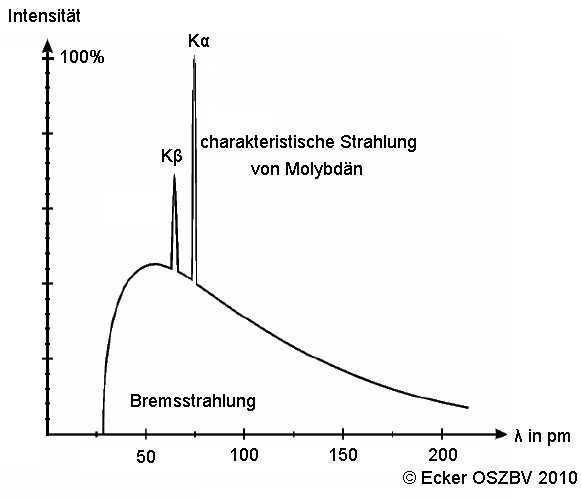
\includegraphics[scale = 0.55]{images/linienspec.png}
				\caption{Röntgenspektrum einer Röntgenröhre unter Verwendung einer Molybdän-Anode \\ Quelle: \refSpektrum}
				\label{fig:brems-spektrum}
			\end{figure}

			Aus Gründen der hohen Anregungsenergien und damit verbundenen hohen Röhrenspannungen zur Erzeugung der $K$-Strahlung schwerer Elemente spielen auch die energieärmeren $L$-Linien eine wesentliche Rolle.

		% subsubsection charakteristische_röntgenlinien (end)

		\subsection{Absorption und Filterung}
		\label{ssec:filterung}
		
			Zur genauen Analyse der Struktur eines Kristalls möchte man im idealen Falle monochromatische Röntgenstrahlung verwenden.
			Durch diese Vereinfachung werden die theoretischen Gleichungen analytisch berechenbar und leicht anwendbar.
			Im vorigen Abschnitt wurde gezeigt, dass im realen Fall keine monochromatische Strahlung vorliegt sondern ein kontinuierliches Bremsspektrum und mehrere $K$-Linien.

			Die Bremsstrahlung kann für die hier betrachteten Fälle vernachlässigt werden, da deren Intensität im Vergleich zu der der $K$-Linien gering ist.
			In Abbildung \ref{fig:brems-spektrum} ist ersichtlich, dass für Molybdän zwei dicht beieinander liegende $K$-Linien mit großer Intensität im Röntgenspektrum erscheinen.
			Dies führt zu verschiedenen Beugungsmustern durch welche die Bestimmung der Gitterkonstanten erschwert oder auch unmöglich wird.
			Deshalb ist es notwendig einen Filter zu verwenden, der eine der beiden $K$-Linien absorbiert.

			Röntgenstrahlen interagieren mit Materie, welche von ihnen durchstrahlt wird, auf drei verschiedenen Wegen.
			Photoabsorption wird durch den Photoeffekt hervorgerufen und kann als inelastischer Stoß betrachtet werden.
			Compton-Streuung ist durch den Compton-Effekt erklärbar.
			Sie kann als elastische Streuung modelliert werden und tritt dominierend für höhere Energien eines jeweiligen Quants auf.
			Bei geringeren Energien tritt ebenfalls eine Form der elastischen Impulsübertragung auf, welche auch als Rayleigh-Streuung bekannt ist.
			Diese drei Wechselwirkungen sind näherungsweise unabhängig von auftretenden Bindungsstrukturen der Elemente, weil Bindungsenergien wesentlich geringer sind, als die Energien der Röntgenstrahlung.
			Ein typisches Absorptionsspektrum ist in Abbildung \ref{fig:x-ray-absorp-spec} zu sehen.

			\urldef{\refXRayAbSpec}\url{http://cpb.iphy.ac.cn/article/2015/cpb_24_8_086101/cpb142671f4_hr.jpg}
			\begin{figure}[htb]
				\centering
				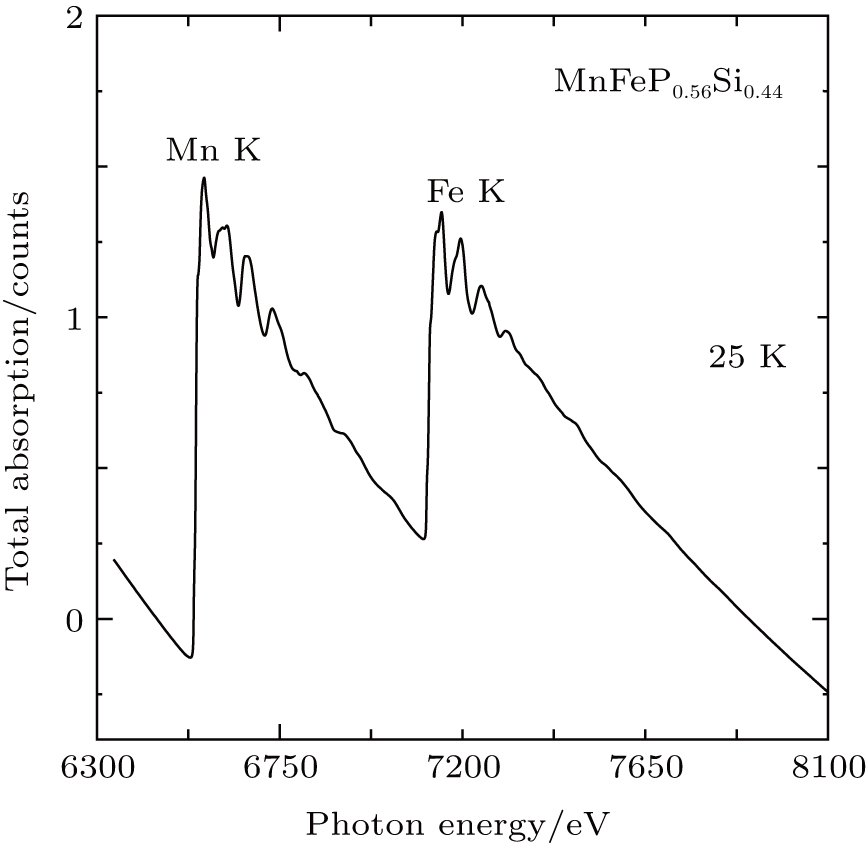
\includegraphics[scale=1.1]{images/x-ray-absorption-spec.jpg}
				\caption{Beispiel eines Röntgenabsorptionsspektrum \\ Quelle: \refXRayAbSpec}
				\label{fig:x-ray-absorp-spec}
			\end{figure}

			Deutlich wird, dass sogenannte Absorptionskanten auftreten, bei welchen das Spektrum nicht stetig verläuft.
			Für Röntgenenergien nahe der Bindungsenergien von Elektronen innerer Schalen treten aufgrund des Photoeffekts abrupte Änderungen der Absorptionswahrscheinlichkeit auf.
			Dieses Phänomen wird in Form von verschiedenen Kanten sichtbar.

			Diese Absorptionskanten können nun ausgenutzt werden, um eine oder mehrere der charakteristischen Linien im Röntgenspektrum zu filtern.
			Abbildung \ref{fig:x-ray-filter} stellt ein Beispiel für eine Molybdän-Anode dar.
			Das verwendete Filtermaterial ist Zirconium, dessen Absorptionskante genau zwischen der $K_\alpha$- und $K_\beta$-Linie von Molybdän liegt.
			Das Resultat ist ein Spektrum, indem die $K_\beta$-Linie stark gedämpft wurde.
			Für die Messung selbst wurde eben dieses Prinzip für eine Kupfer-Anode durch Verwendung eines Nickel-Filters angewandt.

			\urldef{\refFilter}\url{http://clay.uga.edu/courses/8550/BetaFilter.png}
			\begin{figure}[htb]
				\centering
				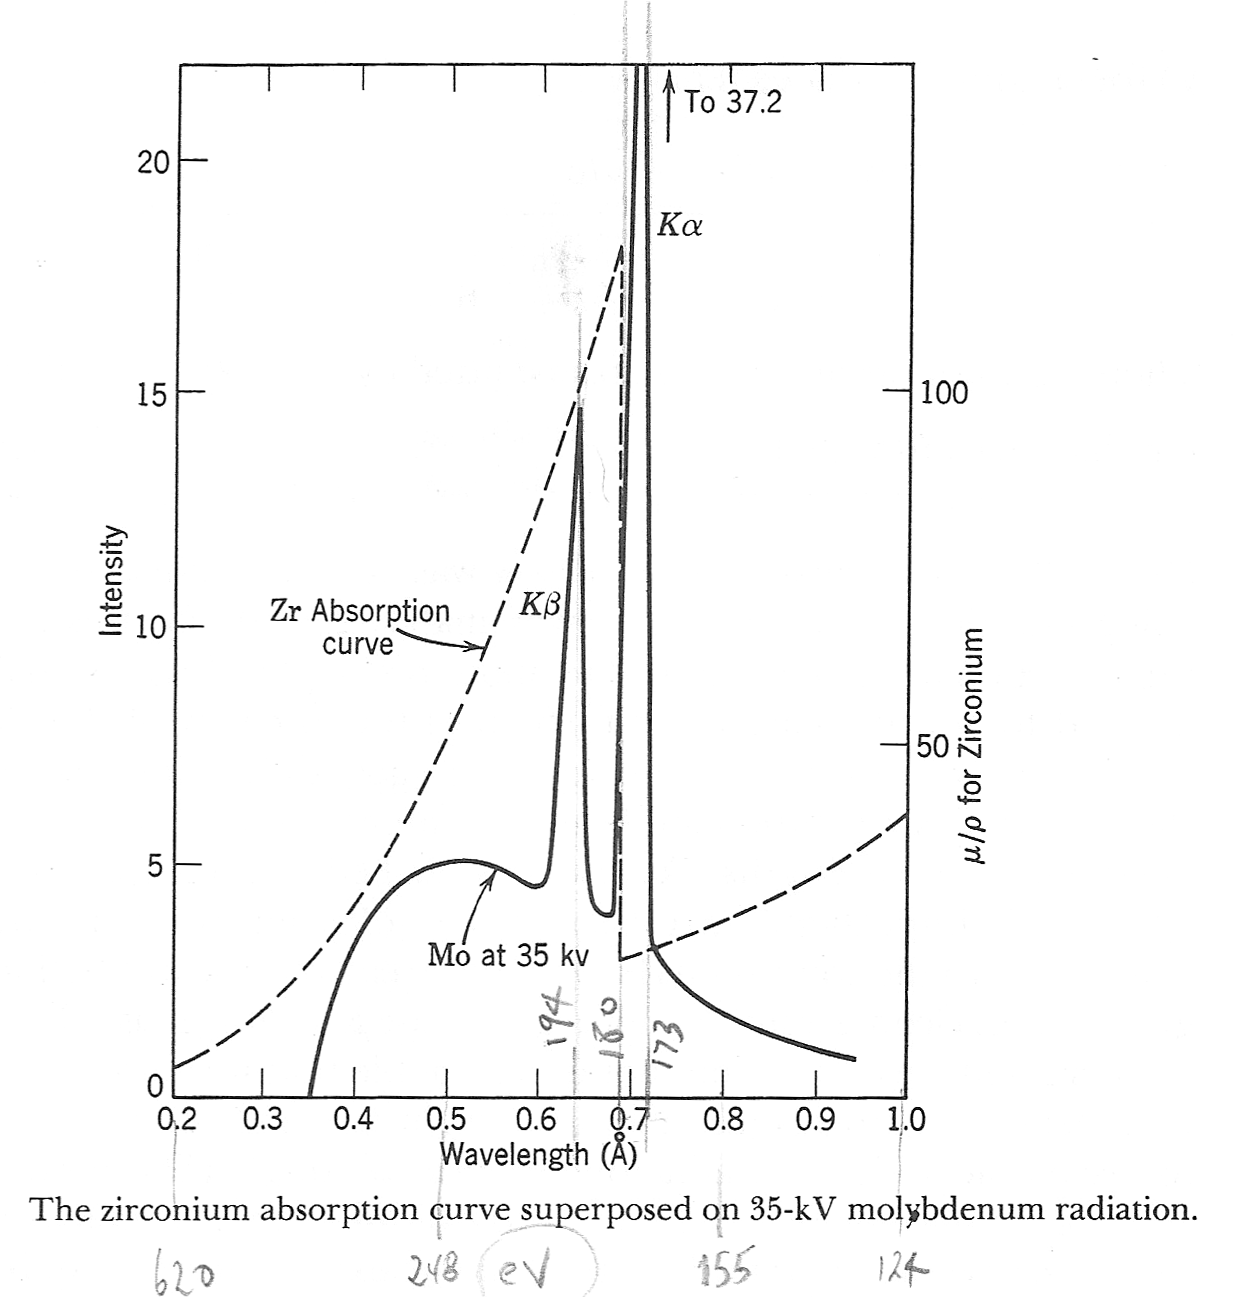
\includegraphics[scale=1]{images/BetaFilter.png}
				\caption{Röntgenspektrum einer Molybdän-Anode und Absorptionsspektrum von Zirconium --- Die Lage der Absorptionskante ermöglicht die alleinige Verwendung der $K_\alpha$-Linie von Molybdän. \\ Quelle: \refFilter}
				\label{fig:x-ray-filter}
			\end{figure}
		
		% subsection filterung

	% subsection erzeugung_von_röntgenstrahlung (end)

	\subsection{Kristallsymmetrie}
	\label{ssec:symmetrie}
	
		Im hier durchgeführten Versuch sind nicht alle Eigenschaften eines Kristallgitters unbekannt.
		Es werden zum Beispiele weder hexagonale noch trikline Kristalle untersucht.
		Die folgende Theorie wird sich deshalb auf die einfacheren Fälle von kubischen, tetragonalen und orthorhombischen Kristallen beschränken.

		Statt also drei verschiedene Gitterkonstanten $a,b,c$ und drei verschiedene Winkel $\alpha,\beta,\gamma$ zu betrachten, werden alle Winkel durch die folgende Bedingung idealisiert.
		\[
			\alpha = \beta = \gamma = \frac{\pi}{2} = 90^\circ
		\]
		Für die Beugung von Röntgenstrahlung an Kristallgittern bilden also nur die drei Gitterkonstanten Freiheitsgrade.
		Dies ermöglicht in den weiteren Abschnitten eine elementare Theorie.
	
	% subsection symmetrie

	\subsection{Beugung von Röntgenstrahlen in Kristallgittern} % (fold)
	\label{sub:beugung_von_rntgenstrahlen_in_kristallgittern}
		
		Trifft Röntgenstrahlung als elektromagnetische Welle auf die Elektronen eines Atoms so regt es diese zu Schwingungen an.
		Durch diesen Effekt angeregte Elektronen werden entsprechend des Huygensschen Prinzips zum Ausgangspunkt einer Röntgenwelle.
		Die Welle wird mit anderen Worten gebeugt.
		Sekundäre Kugelwellen breiten sich im Kristall aus und überlagern einander, wobei konstruktive Interferenz nur für Flächen gleicher Phase auftritt.
		Diese wiederum lassen sich als Tangenten an die Kugelfronten konstruieren, wie es in Abbildung \ref{fig:wellenfront} gezeigt ist.

		\urldef{\refWellenfront}\url{https://elearning.physik.uni-frankfurt.de/data/FB13-PhysikOnline/lm_data/lm_324/daten/bild_4/10_0060.gif}
		\begin{figure}[htb]
			\centering
			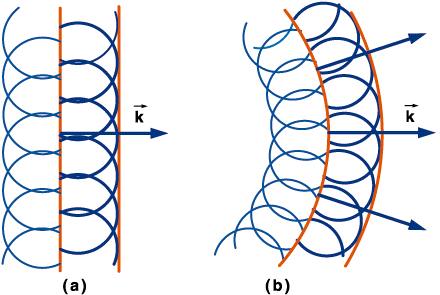
\includegraphics[scale=0.5]{images/wellenfront.png}
			\caption{schematische Darstellung des Huygensschen Prinzips für eine ebene Welle und eine Kugelwelle \\ Quelle: \refWellenfront}
			\label{fig:wellenfront}
		\end{figure}

		Da sehr viele Atome angeregt werden und dementsprechend auch sehr viele Sekundärwellen interferieren, sind die konstruktiv interferierenden Strahlen sehr scharf auf einen kleinen Raumwinkel begrenzt.

		\subsubsection{Laue-Bedingungen}
		\label{sssec:laue-bedingungen}

			\urldef{\refLaue}\url{https://upload.wikimedia.org/wikipedia/commons/5/53/Laue-Bedingung.png}
			\begin{figure}[tb]
				\centering
				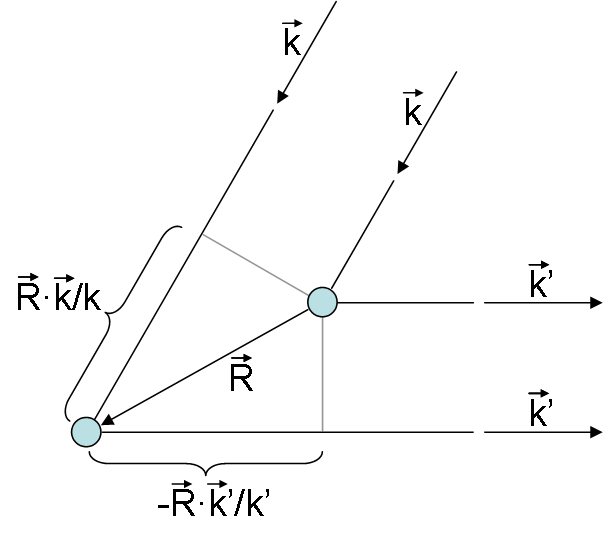
\includegraphics[scale=0.7]{images/Laue-Bedingung.png}
				\caption{Skizze zweier Streuzentren zur Bestimmung der Laue-Bedingungen \\ Quelle: \refLaue}
				\label{fig:laue-bedingungen}
			\end{figure}

			Der Abstand zweier Streuzentren oder auch Gitterpunkten kann als Gittervektor $\bf{R}$ dargestellt werden.
			Es sei nun $\bf{k}$ der Wellenvektor der einfallenden Strahlung und $\bf{k}^\prime$ der der gestreuten Welle mit
			\[
				\norm{\bf{k}} = \norm{\bf{k}^\prime}
			\]
			Anhand von Abbildung \ref{fig:laue-bedingungen} erkennt man leicht, dass sich der Gangunterschied $\Delta x$ aus der nachstehenden Gleichung ergibt.
			\[
				\Delta x = \frac{\angleb{\bf{R},\bf{k}}}{\norm{\bf{k}}} - \frac{\angleb{\bf{R},\bf{k}^\prime}}{\norm{\bf{k}^\prime}}
			\]

			Für konstruktive Interferenz muss der Gangunterschied gerade ein ganzzahliges Vielfaches der Wellenlänge $\lambda = 2\pi/\norm{\bf{k}}$ der vorhandenen Röntgenstrahlung sein.
			Es muss also ein $m\in\SZ$ geben, sodass
			\[
				\Delta x = m\lambda \quad \implies \quad \mathbf{R}(\mathbf{k}-\mathbf{k}^\prime) = 2\pi m
			\]
			Diese Bedingung ist aber gerade äquivalent zu 
			\[
				\tcboxmath{ \exp\boxb{ \mathbf{R}(\mathbf{k}-\mathbf{k}^\prime) } = 1 }
			\]
			Man erhält also genau dann konstruktive Interferenz, wenn die Änderung des Wellenvektors $\bf{k}$ ein reziproker Gittervektor ist.

			Seien nun $a,b,c$ wieder die Gitterkonstante des Kristalls mit zugehörigen Gittervektoren $\bf{a},\bf{b},\bf{c}$.
			Für diesen Fall schreiben sich die Laue-Gleichungen mit $h,k,l\in\SZ$ in der folgenden Form.
			\begin{alignat*}{3}
				a (\cos \overline{\varphi}_a - \cos \varphi_a ) &=&&\ h \lambda \\
				b (\cos \overline{\varphi}_b - \cos \varphi_b ) &=&&\ k \lambda \\
				c (\cos \overline{\varphi}_c - \cos \varphi_c ) &=&&\ l \lambda  
			\end{alignat*}
			Dabei stehen $\varphi_a$,$\varphi_b$,$\varphi_c$ für die Winkel des einfallenden Strahls im Bezug zum jeweiligen Gittervektor $\bf{a},b,c$.
			Analog beschreiben $\overline{\varphi}_a$,$\overline{\varphi}_b$,$\overline{\varphi}_c$ die Winkel des gebeugten Strahls.
		
		% subsubsection laue-bedingungen

		\subsubsection{Bragg-Bedingung}
		\label{sssec:bragg}		

			Alle gerade genannten Gleichungen sind äquivalent zur Bragg-Bedingung.
			Wählt man $n\in\SN$ und sei $d_{hkl}$ der Abstand zweier Netzebenen, welche durch die Millerschen Indizes $(hkl)$ beschrieben werden, so ergibt sich mithilfe des Winkels $\vartheta$ zwischen Röntgenstrahl und Gitterebene
			\[
				\tcboxmath{n \lambda = 2 d_{hkl} \sin \vartheta}
			\]
			$\vartheta$ wird der Glanz- oder auch Bragg-Winkel genannt.
			Jede Netzebene im Kristall ist somit in der Lage einen Beugungsreflex zu erzeugen.
			Die Reflexe liegen umso weiter außen, je näher die Netzebenen zusammenliegen.

			Nach Indizierung der Reflexe mit den oben beschriebenen ganzen Zahlen $h,k,l$ kann man $d_{hkl}$ berechnen.
			\[
				\tcboxmath{d_{hkl} = \boxb{ \curvb{\frac{h}{a}}^2 + \curvb{\frac{k}{b}}^2 + \curvb{\frac{l}{c}}^2 }^{-\frac{1}{2}}}
			\]
		
		% subsubsection bragg

	% subsection beugung_von_röntgenstrahlen_in_kristallgittern (end)

	\subsection{Drehkristallverfahren} % (fold)
	\label{sub:drehkristallverfahren}
		
		Wie in Abschnitt \ref{sub:beugung_von_rntgenstrahlen_in_kristallgittern} gezeigt, kann man anhand der Beugungsreflexe Rückschlüsse über die Gitterkonstante des untersuchten Kristalls ziehen.
		Um jedoch Beugungsreflexe zu erhalten, müssen die Laue-Bedingungen bezüglich Wellenlänge und Winkel erfüllt sein.
		Dafür gibt es verschiedene Strategien.
		Beim Drehkristall-Verfahren wird möglichst monochromatische Strahlung aus der $K_\alpha$-Linie eines gegebenen Elements verwendet und der Winkel $\varphi$ zwischen Strahl und Kristall beständig durch Drehung verändert.
		Durch dieses Vorgehen wird mehrmals der Glanzwinkel für verschiedene Beugungsordnungen erreicht.
		Durch einen Lichtfilm können so entstehende Beugungsreflexe über die Zeit zur späteren Auswertung festgehalten werden.

		\urldef{\refDrehkristall}\url{https://upload.wikimedia.org/wikipedia/commons/9/93/Drehkristall.png}
		\begin{figure}[htb]
			\centering
			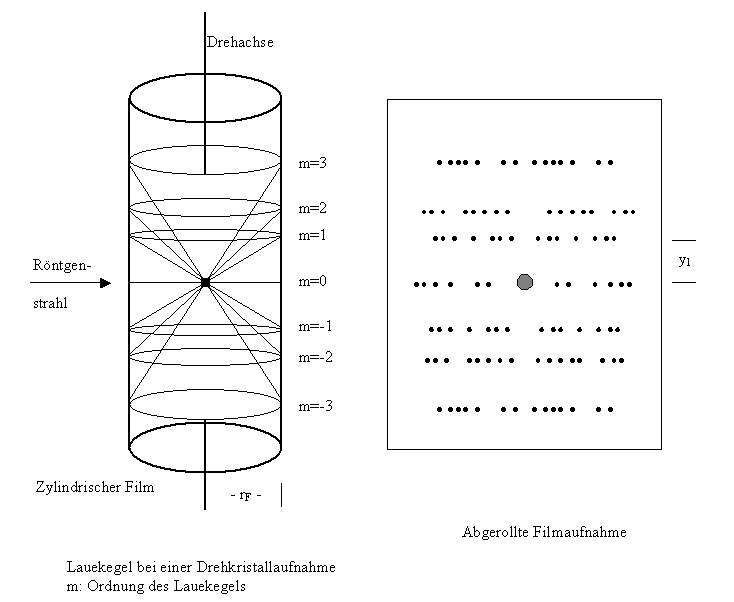
\includegraphics[scale=0.5]{images/Drehkristall.png}
			\caption{Schema zum Aufbau und Vorgehen des Drehkristallverfahrens \\ Quelle: \refDrehkristall}
			\label{fig:scheme-drehkristall}
		\end{figure}

		Im Normalfall liegt die Drehachse senkrecht zum Primärstrahl ($\varphi = 90^\circ$), dadurch vereinfachen sich die Laue Bedingungen zu
		\[ a \cos \overline{\varphi} = h \lambda \]
		Die abgebeugten Strahlen liegen demnach auf einem Kreiskegel mit dem Öffnungswinkel $2 \overline{\varphi} $.
		Auf dem zylindrisch angeordneten Film sind die Reflexe für ein festes $h$ somit auf parallelen Schichtlinien.
		Bezeichnet $e / 2$ den Abstand der ersten Schichtlinie zum Äquator, so lässt sich bei gegebenen Kameraradius $r$ der Glanzwinkel für die Drehachse bestimmen zu
		\[ \tan (90^\circ - \overline{\varphi}) = \frac{e}{2r} \]
		Dann folgt für die Gitterkonstante in Richtung der Drehachse
		\[ a = \frac{h \lambda}{\cos \overline{\varphi} } \quad \implies \quad a = \frac{h\lambda}{\sin\arctan \frac{e}{2r}} \]

	% subsection drehkristallverfahren (end)

% section grundlagen (end)